\documentclass[article]{jss}\usepackage{graphicx, color}
%% maxwidth is the original width if it is less than linewidth
%% otherwise use linewidth (to make sure the graphics do not exceed the margin)
\makeatletter
\def\maxwidth{ %
  \ifdim\Gin@nat@width>\linewidth
    \linewidth
  \else
    \Gin@nat@width
  \fi
}
\makeatother

\definecolor{fgcolor}{rgb}{0, 0, 0}
\newcommand{\hlnumber}[1]{\textcolor[rgb]{0.501960784313725,0,0.501960784313725}{#1}}%
\newcommand{\hlfunctioncall}[1]{\textcolor[rgb]{0,0.501960784313725,0.752941176470588}{\textbf{#1}}}%
\newcommand{\hlstring}[1]{\textcolor[rgb]{0.650980392156863,0.52156862745098,0}{#1}}%
\newcommand{\hlkeyword}[1]{\textcolor[rgb]{0.733333333333333,0.474509803921569,0.466666666666667}{\textbf{#1}}}%
\newcommand{\hlargument}[1]{\textcolor[rgb]{0,0,0}{#1}}%
\newcommand{\hlcomment}[1]{\textcolor[rgb]{1,0.501960784313725,0}{#1}}%
\newcommand{\hlroxygencomment}[1]{\textcolor[rgb]{1,0.501960784313725,0}{#1}}%
\newcommand{\hlformalargs}[1]{\textcolor[rgb]{0,0,0}{#1}}%
\newcommand{\hleqformalargs}[1]{\textcolor[rgb]{0,0,0}{#1}}%
\newcommand{\hlassignement}[1]{\textcolor[rgb]{0,0,0}{#1}}%
\newcommand{\hlpackage}[1]{\textcolor[rgb]{0.501960784313725,0.501960784313725,0.752941176470588}{\textbf{#1}}}%
\newcommand{\hlslot}[1]{\textcolor[rgb]{0,0,0}{\textit{#1}}}%
\newcommand{\hlsymbol}[1]{\textcolor[rgb]{1,0,0.501960784313725}{#1}}%
\newcommand{\hlprompt}[1]{\textcolor[rgb]{0,0,0}{#1}}%

\usepackage{framed}
\makeatletter
\newenvironment{kframe}{%
 \def\at@end@of@kframe{}%
 \ifinner\ifhmode%
  \def\at@end@of@kframe{\end{minipage}}%
  \begin{minipage}{\columnwidth}%
 \fi\fi%
 \def\FrameCommand##1{\hskip\@totalleftmargin \hskip-\fboxsep
 \colorbox{shadecolor}{##1}\hskip-\fboxsep
     % There is no \\@totalrightmargin, so:
     \hskip-\linewidth \hskip-\@totalleftmargin \hskip\columnwidth}%
 \MakeFramed {\advance\hsize-\width
   \@totalleftmargin\z@ \linewidth\hsize
   \@setminipage}}%
 {\par\unskip\endMakeFramed%
 \at@end@of@kframe}
\makeatother

\definecolor{shadecolor}{rgb}{.97, .97, .97}
\definecolor{messagecolor}{rgb}{0, 0, 0}
\definecolor{warningcolor}{rgb}{1, 0, 1}
\definecolor{errorcolor}{rgb}{1, 0, 0}
\newenvironment{knitrout}{}{} % an empty environment to be redefined in TeX

\usepackage{alltt}
\usepackage[utf8]{inputenc}
\usepackage{amsmath}
\usepackage{dsfont}
\usepackage{tabularx}
\frenchspacing

\newcommand{\atanh}{\text{atanh}}

%%%%%%%%%%%%%%%%%%%%%%%%%%%%%%
%% declarations for jss.cls %%%%%%%%%%%%%%%%%%%%%%%%%%%%%%%%%%%%%%%%%%
%%%%%%%%%%%%%%%%%%%%%%%%%%%%%%

%% almost as usual
\author{Stefan Siegert\\University of Exeter}
\title{Ensemble Forecast Verification Functions Implemented in the \proglang{R} Package \pkg{SpecsVerification}}
\Shorttitle{\pkg{SpecsVerification}: R Functions for Ensemble Verification} %% a short title (if necessary)
\Plainauthor{Stefan Siegert} %% comma-separated
\Plaintitle{Forecast Verification Methods Implemented in the R package SpecsVerification: Ensemble Scores, Comparative Verification, and Uncertainty Quantification}

%% an abstract and keywords
\Abstract{

Forecast verification, the comparison of retrospective forecasts to observations, is a common task at institutions that develop and issue forecasts, such as climate centers.
To assess forecast uncertainty, ensembles of forecasts initialised from perturbed initial conditions are routinely issued.
In recent years, advances have been made in statistical methodology for ensemble forecast verification, in particular to estimate the finite-ensemble effect on verification scores.
This paper summarises statistical methodology to account for finite-ensemble effects in ensemble verification, to compare the quality of ensemble forecasts with different numbers of ensemble members, and to quantify uncertainty in forecast verification results.
Implementations of the methods are freely available in the \proglang{R} package \pkg{SpecsVerification}.

}
\Keywords{ensemble forecasting, forecast verification, finite-ensemble effect, comparative verification, uncertainty quantification, \proglang{R}}
\Plainkeywords{ensemble forecasting, forecast verification, finite-ensemble effect, comparative verification, uncertainty quantification, R} %% without formatting
%% at least one keyword must be supplied

%% publication information
%% NOTE: Typically, this can be left commented and will be filled out by the technical editor
%% \Volume{50}
%% \Issue{9}
%% \Month{June}
%% \Year{2012}
%% \Submitdate{2012-06-04}
%% \Acceptdate{2012-06-04}

%% The address of (at least) one author should be given
%% in the following format:
\Address{
  Stefan Siegert\\
  Statistical Science Group\\
  University of Exeter\\
  Exeter, EX4 4QF, United Kingdom\\
  E-mail: \email{Stefan.Siegert@exeter.ac.uk}\\
  URL: \url{http://emps.exeter.ac.uk/mathematics/staff/ss610}
}


%% end of declarations %%%%%%%%%%%%%%%%%%%%%%%%%%%%%%%%%%%%%%%%%%%%%%%

% initialise R session and knitr


\IfFileExists{upquote.sty}{\usepackage{upquote}}{}


\begin{document}

%% Note that you should use the \pkg{}, \proglang{} and \code{} commands.
% \section[About Java]{About \proglang{Java}}
%% Note: If there is markup in \(sub)section, then it has to be escape as above.


\section{Introduction}

%{\bf Ensemble forecasting general}
An ensemble forecast is a collection of forecasts for the same target.
The ensemble members usually differ due to differences in initial conditions, boundary conditions, model physics and background information \citep{gneiting2005atmospheric, leutbecher2008ensemble}.
Ensemble forecasting is today operationally used in weather and climate forecasting to explore the chaotic divergence of nonlinear systems, and to estimate forecast uncertainty.
To evaluate the reliability and predictive skill of ensemble forecasts, the forecasts have to be compared to their verifying observations of the real world.
%
%{\bf Forecast verification general}
The comparison of forecasts with their verifying observations is commonly referred to as forecast verification \citep{jolliffe2012forecast}.
A verification measure is thus a function that depends on an archive $D=\{x_t, y_t\}_{t=1}^N$ of past forecasts $x_t$ and verifying observations $y_t$.
The archive $D$ is also called a hindcast data set.
A variety of verification measures exists to assess the quality of different forecast products, such as deterministic forecasts, probabilistic forecasts, ensemble forecasts, univariate or multivariate forecasts, and gridded or unevenly spaced spatial forecasts.


%{\bf Finite size effect in ensemble verification}
The \proglang{R} package \pkg{SpecsVerification} documented in this paper focuses primarily on verification scores for ensemble forecasts.
It is known that verification measures can depend systematically on the ensemble size; everything else being equal, large ensembles achieve better average scores than small ensembles \citep{buizza1998impact}.
Since hindcast experiments with state-of-the-art climate models are computationally expensive, 
new model configurations are often verified on small ensemble sizes.
Large ensembles are only generated in forecast mode.
But if verification measures depend on the ensemble size, the skill calculated for the hindcast experiment is not representative of the skill that an operational forecast ensemble with more members would achieve.
A number of verification scores have been proposed in the past to estimate the finite ensemble effect.
The main contribution of this paper is to summarise ensemble verification scores, and document their implementation in the \proglang{R} statistical programming environment.
The package \pkg{SpecsVerification} contains functions to calculate verification scores, compare verification scores, and quantify uncertainty.




\begin{table}
\renewcommand{\arraystretch}{1.5}
\caption{Overview of verification functions implemented in \pkg{SpecsVerification}, and their application.}
\begin{tabular}{lll}
&&\\
\textsc{Function} & \textsc{Long name} & \textsc{Applies to} \\
\hline
\code{AbsErr} & Absolute error Score$^*$ & \vtop{\hbox{\strut Deterministic forecasts of continuous}\hbox{\strut observations}}\\
\code{Auc} & Area under the ROC curve & \vtop{\hbox{\strut Probability forecasts of binary}\hbox{\strut observations}}\\
\code{AucDiff} & \vtop{\hbox{\strut Difference between two areas}\hbox{\strut under the ROC curve}} & \vtop{\hbox{\strut Two competing probability forecasts}\hbox{\strut for the same binary observations}}\\
\code{Corr} & Correlation coefficient & \vtop{\hbox{\strut Deterministic forecasts of continuous}\hbox{\strut observations}}\\
\code{CorrDiff} & \vtop{\hbox{\strut Difference between two}\hbox{\strut correlation coefficients}} & \vtop{\hbox{\strut Two competing deterministic forecasts}\hbox{\strut for the same continuous observations }}\\
\code{DressCrps} & \vtop{\hbox{\strut Continuous ranked probability}\hbox{\strut score for dressed ensembles$^*$}} & \vtop{\hbox{\strut Ensemble forecasts of continuous}\hbox{\strut observations}}\\
\code{DressIgn} & \vtop{\hbox{\strut Ignorance score for}\hbox{\strut dressed ensembles$^*$}} & \vtop{\hbox{\strut Ensemble forecasts of continuous}\hbox{\strut observations}}\\
\code{EnsBrier} & Ensemble-adjusted Brier score$^*$ & \vtop{\hbox{\strut Ensemble forecast of binary}\hbox{\strut observations }}\\
\code{EnsCrps} & \vtop{\hbox{\strut Ensemble-adjusted continuous}\hbox{\strut ranked probability score$^*$}} & \vtop{\hbox{\strut Ensemble forecasts of continuous}\hbox{\strut observations}}\\
\code{EnsRps} & \vtop{\hbox{\strut Ensemble-adjusted ranked}\hbox{\strut probability score$^*$}} & \vtop{\hbox{\strut Ensemble forecasts of categorical}\hbox{\strut observations }}\\
\code{EnsQs} & \vtop{\hbox{\strut Ensemble-adjusted quadratic}\hbox{\strut score$^*$}} & \vtop{\hbox{\strut Ensemble forecasts of categorical}\hbox{\strut observations}}\\
\code{GaussCrps} & \vtop{\hbox{\strut Continuous ranked probability}\hbox{\strut score for Normal distributions$^*$}} & \vtop{\hbox{\strut Probability forecasts of continuous}\hbox{\strut observations}}\\
\code{PlotRankhist} & Plot a rank histogram & see \code{Rankhist} \\
\code{Rankhist} & Calculate a rank histogram & \vtop{\hbox{\strut Ensemble forecasts of continuous}\hbox{\strut observations }}\\
\code{ReliabilityDiagram} & \vtop{\hbox{\strut Calculate and plot a}\hbox{\strut reliability diagram}} & \vtop{\hbox{\strut Probability forecasts of binary}\hbox{\strut observations }}\\
\code{ScoreDiff} & \vtop{\hbox{\strut Calculate a score difference}\hbox{\strut and assess uncertainty}} & All scores marked with a $^*$\\
\code{SkillScore} & \vtop{\hbox{\strut Calculate a skill score}\hbox{\strut and assess uncertainty}} & All scores marked with a $^*$\\
\code{TestRankhist} & \vtop{\hbox{\strut Statistical tests of}\hbox{\strut a rank histogram}} & see \code{Rankhist} \\
\code{SqErr} & Squared error score$^*$ & \vtop{\hbox{\strut Deterministic forecasts of continuous}\hbox{\strut observations}}\\
\end{tabular}
\end{table}

\section{Forecast and observation data}


 
\pkg{SpecsVerification} includes the data set \code{eurotempforecast} of seasonal temperature ensemble forecasts and verifying observations.
The forecasts 24-member ensembles of near-surface air temperatures produced by the NCEP climate forecast system version 2 \citep{saha2014ncep}, initialised between 11 April and 6 May each year from 1983--2009 ($N=27$), and averaged over the region limited by latitudes $30^\circ$N -- $75^\circ$N and longitudes $12.5^\circ$W -- $42.5^\circ$E, and over the months June-July-August, i.e., the lead time is about 1--3 months.
Data from the NCEP climate forecast system reanalysis \citep{saha2010ncep} was taken as verifying observations.
All data was downloaded through the ECOMS user data gateway R-interface \citep{ecoms2015}.
Ensemble members and observation data are plotted as time series in Figure \ref{gfs-plot}.

\begin{knitrout}
\definecolor{shadecolor}{rgb}{0.933, 0.933, 0.933}\color{fgcolor}\begin{kframe}
\begin{alltt}
\hlfunctioncall{data}(eurotempforecast)
R   <- \hlfunctioncall{ncol}(ens)
yrs <- \hlfunctioncall{as.numeric}(\hlfunctioncall{names}(obs))
N   <- \hlfunctioncall{length}(obs)
\end{alltt}
\end{kframe}
\end{knitrout}




\begin{figure}
\begin{center}
%
\begin{knitrout}
\definecolor{shadecolor}{rgb}{0.933, 0.933, 0.933}\color{fgcolor}\begin{kframe}
\begin{alltt}
\hlfunctioncall{par}(las=1, cex=0.7, mgp=\hlfunctioncall{c}(3, 1, 0), mar=\hlfunctioncall{c}(2,4,1,1))
\hlfunctioncall{matplot}(yrs, ens, ylab=\hlstring{"temp [C]"}, pch=1, col=\hlfunctioncall{gray}(.5))
\hlfunctioncall{points}(yrs, obs, pch=15, cex=1.5)
\end{alltt}
\end{kframe}
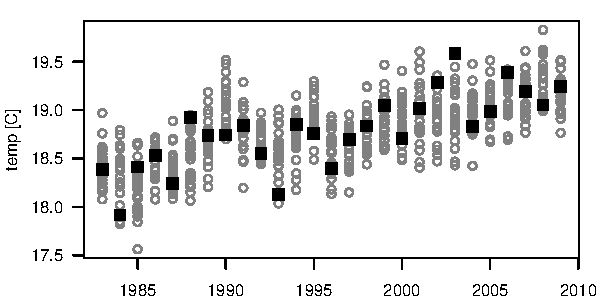
\includegraphics[width=\maxwidth]{figure/gfs-plot} 

\end{knitrout}

%
\end{center}
\caption{Seasonal European temperature ensemble forecasts (circles) and verifying observations (squares).}
\label{gfs-plot}
\end{figure}


All functions in \pkg{SpecsVerification} that analyse ensemble forecast data, assume that archives of $N$ instances of $R$-member ensemble forecasts, are represented by $N\times R$ matrices.
The data shown in Figure \ref{gfs-plot} depicts 27 years or 24-member ensemble forecasts, and is thus a \proglang{R} matrix with $27$ rows and $24$ columns.


Real-valued forecasts and real-valued observations are saved as \proglang{R} matrix \code{ens} and \proglang{R} vector \code{obs}. 
The continuous data in \code{ens} and \code{obs} was used to derive binary and categorical forecasts and observations (matrices \code{ens.bin} and \code{ens.cat}, and vectors \code{obs.bin} and \code{obs.cat}).
The binary forecasts, were generated by asking "Will this year's summer be warmer than last year's"?
The binary observation at time index $t$ is equal to one if the temperature in the corresponding year exceeds the temperature of the previous year, and zero otherwise.
The individual ensemble members were transformed equivalently, by comparing the $r$th ensemble member in year $t$ to the observation in year $t-1$.
Categorical forecasts and observations were generated by asking "Will this year's temperature be similar to last year's temperature (within a 0.5K range), colder, or warmer?"
Ensemble members and the observation thus fall into one of 3 categories: Category 1 if the temperature that is less than $0.25K$ colder than the previous year, category 2 if the temperature is within $\pm 0.25K$ of the previous year, and category 3 if it is more than $0.25K$ warmer.
In addition, the vector \code{obs.lag} is provided, containing 1-year lagged observed temperatures.
For example, continuous, binary and categorical observations and forecasts for the year 2001 are 

\begin{knitrout}
\definecolor{shadecolor}{rgb}{0.933, 0.933, 0.933}\color{fgcolor}\begin{kframe}
\begin{alltt}
\hlfunctioncall{rbind}(
continuous = \hlfunctioncall{c}(obs=obs[\hlstring{"2001"}], ens[\hlstring{"2001"}, 1:5]),
binary     = \hlfunctioncall{c}(obs=obs.bin[\hlstring{"2001"}], ens.bin[\hlstring{"2001"}, 1:5]),
categorical = \hlfunctioncall{c}(obs=obs.cat[\hlstring{"2001"}], ens.cat[\hlstring{"2001"}, 1:5]))
\end{alltt}
\begin{verbatim}
##             obs.2001 Member_1 Member_2 Member_3 Member_4 Member_5
## continuous     19.01    18.65    18.96    19.23    18.41    18.81
## binary          1.00     0.00     1.00     1.00     0.00     1.00
## categorical     3.00     2.00     3.00     3.00     1.00     2.00
\end{verbatim}
\end{kframe}
\end{knitrout}




\section{Ensemble-adjusted verification scores}



\subsection{Binary ensemble forecasts}

This subsection outlines the theory behind ensemble-adjusted verification scores, using probabilistic forecasts of binary events.
One of the most common verification measures for probabilistic forecasts of binary events is the Brier score \citep{brier1950verification}.
Suppose a probability forecast $p_t \in [0,1]$ is issued at time $t$ for a binary (yes/no) event.
The occurrence (non-occurrence) of the event is coded as $y_t=1$ ($y_t=0$). 
The Brier score is given by the squared difference between forecast and observation:
%
\begin{equation}
s_{B}(p_t, y_t) = (p_t - y_t)^2
\end{equation}
%
The Brier score is negatively oriented: Lower scores indicate better forecasts.
The Brier score is a strictly proper verification score, meaning that the expected score obtains its minimum value if and only if the observation $y_t$ is a random draw from $p_t$ \citep{gneiting2007strictly}.


Suppose that the probability $p_t$ is unknown, but an ensemble forecast of size $R$ drawn from $p_t$ is available.
Each of the $R$ ensemble members is interpreted as an independent Bernoulli trial with success probability $p_t$.
An unbiased estimator of $p_t$ is given by the fraction $i_t/R$, where $i_t$ is the number of ensemble members that predict the event $y_t=1$.
The Brier score of the probability forecast $i_t/R$ is equal to
%
\begin{equation}
s_{B}\left(\frac{i_t}{R}, y_t\right) = \left(\frac{i_t}{R} - y_t\right)^2
\label{eq:unfair-brier}
\end{equation}
%
and taking expectation over the random variable $i_t \sim Binomial(p_t, R)$, it is shown that \citep{ferro2008effect}
%
\begin{equation}
E\left[s_{B}\left(\frac{i_t}{R}, y_t\right)\right] = s_{B}(p_t, y_t) +\frac{p_t(1-p_t)}{R}.
\label{eq:expec-brier}
\end{equation}
%
That is, the Brier score of $i_t/R$ is a biased estimator of the Brier score of $p_t$.
The expected Brier score of $i_t/R$ is larger (i.e. worse) than the Brier score of $p_t$.
The bias, given by the additional positive term on the rhs of Equation~\ref{eq:expec-brier}, depends on the ensemble size and vanishes for $R\rightarrow\infty$.
The bias can be interpreted as a finite-ensemble penalty: If two ensembles sample their members from the same probability $p_t$, the one with the larger ensemble size obtains the lower (i.e. better) expected Brier score.
This is reasonable since more ensemble members allow for more robust estimation of the true probability $p_t$.
But it is sometimes desirable to correct the finite-ensemble bias.
Suppose, for example, a hindcast ensemble has $R$ members, but future operational forecasts will be made with $R^* > R$ ensemble members, using the same ensemble system. 
Due to the finite-ensemble bias, the score calculated for the $R$-member hindcast ensemble will be a too pessimistic estimate of the expected score of the $R^*$-member forecast ensemble.
An adjustment is desirable that allows to use an $R$ member ensemble to unbiasedly estimate the score of an $R^* \neq R$ member ensemble.


The ensemble-adjusted Brier score, given by \citep{ferro2008effect}
%
\begin{equation}
s_{B}^*(i_t, R, R^*, y_t) = \left(\frac{i_t}{R} - y_t\right)^2 - \left(\frac{1}{R} - \frac{1}{R^*}\right)\frac{i_t(R-i_t)}{R(R-1)}
\label{eq:ens-brier}
\end{equation}
%
includes a correction of the finite-ensemble bias.
The ensemble-adjusted Brier score is, in expectation, equal to the Brier score that would be achieved by an ensemble with $R^*$ members, whose members are sampled from the same probability $p_t$, i.e., 
%
\begin{equation}
E\left[s_{B}^*(i_t, R, R^*, y_t)\right] = (p_t - y_t)^2 + \frac{p_t(1-p_t)}{R^*}.
\end{equation}
%
Setting $R^*=\infty$ yields the fair Brier score \citep{ferro2013fair} which is an unbiased estimator of the Brier score of the underlying (unknown) probability $p_t$.
The ensemble-adjusted Brier score can be used to compare ensemble forecasting systems (e.g. from different climate centers) that use different ensemble sizes.
The score further allows for the extrapolation of the average score of an ensemble forecast system to larger ensemble sizes, e.g., to estimate forecast skill with $R^*$ members based on hindcast skill with $R<R^*$ members.
The \pkg{SpecsVerification} function \code{EnsBrier} calculates the ensemble-adjusted Brier scores of a collection of $N$ ensemble forecasts and their corresponding binary observations. 
The argument \code{R.new} allows for estimation of the score of an arbitrary ensemble size, including \code{R.new=Inf}.


To illustrate the finite ensemble effect, we randomly split the 24-member forecast ensemble \code{ens} into a small 5-member subensemble, and a larger 19-member subensemble, and calculate their unadjusted Brier scores (Equation~\ref{eq:unfair-brier}):
%
\begin{knitrout}
\definecolor{shadecolor}{rgb}{0.933, 0.933, 0.933}\color{fgcolor}\begin{kframe}
\begin{alltt}
i.small <- \hlfunctioncall{sample}(1:R, 5)
i.large <- \hlfunctioncall{setdiff}(1:R, i.small)
\hlfunctioncall{c}(small.ens=\hlfunctioncall{mean}(\hlfunctioncall{EnsBrier}(ens.bin[, i.small], obs.bin)), 
  large.ens=\hlfunctioncall{mean}(\hlfunctioncall{EnsBrier}(ens.bin[, i.large], obs.bin)))
\end{alltt}
\begin{verbatim}
## small.ens large.ens 
##    0.1689    0.1465
\end{verbatim}
\end{kframe}
\end{knitrout}

%
The large subensemble obtains a better average Brier score than the small subensemble, even though both ensembles were produced by the same ensemble forecasting system.
We next adjust the Brier score for the finite ensemble size, by calculating $s_{B}^*$ using $R^*=19$ for both ensembles:
%
\begin{knitrout}
\definecolor{shadecolor}{rgb}{0.933, 0.933, 0.933}\color{fgcolor}\begin{kframe}
\begin{alltt}
\hlfunctioncall{c}(small.ens=\hlfunctioncall{mean}(\hlfunctioncall{EnsBrier}(ens.bin[, i.small], obs.bin, R.new=19)), 
  large.ens=\hlfunctioncall{mean}(\hlfunctioncall{EnsBrier}(ens.bin[, i.large], obs.bin, R.new=19)))
\end{alltt}
\begin{verbatim}
## small.ens large.ens 
##    0.1454    0.1465
\end{verbatim}
\end{kframe}
\end{knitrout}

%
After adjusting for the finite-ensemble bias, the scores are very similar. 
Using the ensemble-adjusted Brier score, we were able to extrapolate the Brier score of a 5-member ensemble to the Brier score that a 19-member ensemble would achieve, produced by the same ensemble forecasting system. 



\subsection{Categorical ensemble forecasts}

Suppose a forecast target that always falls into exactly one out of $K$ disjoint categories.
A probabilistic forecast for this target is the vector $\mathbf{p}_t = (p_{t,1}, \cdots, p_{t,K})$, whose $k$th element equals the forecast probability that the observation will materialise in class $k$.
The verifying observation is vector-valued $\mathbf{y}_t$, where the $k$th element of $\mathbf{y}_t$ is $y_{t,k}=1$ if the $k$th class is observed, and $y_{t,j}=0$ for all $j\neq k$. 
The quadratic score (QS) of the probability forecast $\mathbf{p}_t$ with verifying observation $\mathbf{y}_t$ is given by
%
\begin{equation}
s_{Q}(\mathbf{p}_t, \mathbf{y}_t) = \sum_{k=1}^K \left(p_{t,k} - y_{t,k}\right)^2.
\end{equation}


Now assume an $R$-member categorical ensemble forecast $\mathbf{i}_t$ is issued at time $t$, indicating that $i_{t,k}$ out of $R$ ensemble members have predicted the $k$th category, for $k=1,\cdots,K$.
Using results obtained for the ensemble-adjusted Brier score, \citep[see also][]{ferro2008effect}, the ensemble-adjusted QS is seen to be
%
\begin{equation}
s_{Q}^*(\mathbf{i}_t, R, R^*, \mathbf{y}_t) = \sum_{k=1}^K \left\{ \left(\frac{i_{t,k}}{R} - y_{t,k}\right)^2 - \left(\frac{1}{R} - \frac{1}{R^*}\right) \frac{i_{t,k}(R-i_{t,k})}{R(R-1)}\right\}
\end{equation}
%
The ensemble-adjusted QS is implemented as the function \code{EnsQs} in \pkg{SpecsVerification}.
The function expects the argument \code{ens} to be provided as a $N\times R$ matrix of categorical ensemble forecasts, where \code{ens[t,r]} indicates the category predicted by the $r$th ensemble members at time $t$. 

The QS is invariant under relabelling of the $K$ categories, and therefore insensitive to distance. 
If the observation materialises in class $1$, say, the QS penalises a forecast that puts all probability mass into class $2$ as much as a forecast that puts all probability mass into class $3$.
In forecast forecast problems where the categories convey a natural ordering of the forecast target, such as $\{1$=``no rain'', $2$=``light rain''; $3$=``heavy rain''$\}$, a forecast that predicts class 2 might seem preferable to a forecast that predicts class 3, if class 1 occurs. 

The ranked probability score (RPS) is a version of the QS that is sensitive to distance.
The ensemble forecast vector $\mathbf{i}_t$ is transformed to the cumulated forecast vector $\mathbf{j}_t$, with $k$th element equal to $j_{t,k} = \sum_{l=1}^k i_{t,l}$, and the cumulated observation vector $\mathbf{z}_t$ has $z_{t,k} = \sum_{l=1}^k y_{t,l}$.
The RPS is the QS of the forecast $\mathbf{j}_t$ evaluated on the observation $\mathbf{z}_t$.
Accumulating the elements of $\mathbf{i}_t$ and $\mathbf{y}_t$ nests the $K$ forecast categories within each other. 
Essentially, the forecast is transformed from ``$i_{t,k}$ out of $R$ ensemble members predict category $k$'' to the forecast ``$j_{t,k}$ out of $R$ ensemble members forecast category $k$ \emph{or less}''.
Nesting of forecast categories enables order-sensitivity of the score.
Using results from the previous section, we get the ensemble-adjusted RPS
%
\begin{equation}
s_{R}^*(\mathbf{i}_t, R, R^*, \mathbf{y}_t) = \sum_{k=1}^K \left\{ \left(\frac{j_{t,k}}{R} - z_{t,k}\right)^2 - \left(\frac{1}{R} - \frac{1}{R^*}\right) \frac{j_{t,k}(R-j_{t,k})}{R(R-1)}\right\}
\end{equation}
%
The ensemble-adjusted RPS is implemented as the function \code{EnsRps} in \pkg{SpecsVerification}.
The argument \code{ens} should be provided as for \code{EnsQs}; the nesting of forecast categories is performed internally.



To illustrate the finite-ensemble effect and its adjustment in the QS and RPS, we split the ensemble randomly into a 5-member ensemble and a 19-member ensemble. 
We evaluate the unadjusted QS of the full 24-member ensemble, the unadjusted scores of the small and large subensembles, as well as the QS of the two subensembles adjusted for the size $R^*=24$ of the full ensemble:
%
\begin{knitrout}
\definecolor{shadecolor}{rgb}{0.933, 0.933, 0.933}\color{fgcolor}\begin{kframe}
\begin{alltt}
i.small <- \hlfunctioncall{sample}(1:R, 5)
i.large <- \hlfunctioncall{setdiff}(1:R, i.small)
\hlfunctioncall{cbind}(
 QS = \hlfunctioncall{c}(
  ens           = \hlfunctioncall{mean}(\hlfunctioncall{EnsQs}(ens.cat,            obs.cat)),
  small.ens     = \hlfunctioncall{mean}(\hlfunctioncall{EnsQs}(ens.cat[, i.small], obs.cat)),
  large.ens     = \hlfunctioncall{mean}(\hlfunctioncall{EnsQs}(ens.cat[, i.large], obs.cat)),
  small.ens.adj = \hlfunctioncall{mean}(\hlfunctioncall{EnsQs}(ens.cat[, i.small], obs.cat, R.new=24)),
  large.ens.adj = \hlfunctioncall{mean}(\hlfunctioncall{EnsQs}(ens.cat[, i.large], obs.cat, R.new=24))
 ),
 RPS = \hlfunctioncall{c}(
  ens           = \hlfunctioncall{mean}(\hlfunctioncall{EnsRps}(ens.cat,            obs.cat)),
  small.ens     = \hlfunctioncall{mean}(\hlfunctioncall{EnsRps}(ens.cat[, i.small], obs.cat)),
  large.ens     = \hlfunctioncall{mean}(\hlfunctioncall{EnsRps}(ens.cat[, i.large], obs.cat)),
  small.ens.adj = \hlfunctioncall{mean}(\hlfunctioncall{EnsRps}(ens.cat[, i.small], obs.cat, R.new=24)),
  large.ens.adj = \hlfunctioncall{mean}(\hlfunctioncall{EnsRps}(ens.cat[, i.large], obs.cat, R.new=24))
 )
)
\end{alltt}
\begin{verbatim}
##                   QS    RPS
## ens           0.5782 0.3344
## small.ens     0.6519 0.3719
## large.ens     0.5856 0.3386
## small.ens.adj 0.5815 0.3597
## large.ens.adj 0.5810 0.3378
\end{verbatim}
\end{kframe}
\end{knitrout}

%
The full-ensemble obtains a better score than either of the sub-ensembles and the large subensemble outperforms the small subensemble.
When adjusting scores of the subensembles to $R^*=24$, the scores of the subensembles are more similar to each other, and closer to the score of the full ensemble.
Note that the equality of ensemble-adjusted scores for different ensemble sizes holds only in expectation. 
Empirical averages over finite numbers of hindcasts differ, which explains the differences in the previous analyses.
The reader is referred to \citet{ferro2013fair} for illustrations of convergence by random number experiments.

\subsection{Continuous ensemble forecasts}


If the forecast target is a continuous variable, such as temperature or pressure, the continuous ranked probability score \citep[CRPS;][]{matheson1976scoring} can be used for forecast verification.
If the forecast for the continuous target $y_t$ is given as a cumulative distribution function (cdf) $F_t(x)$, the CRPS is given by 
%
\begin{equation}
s_{C}(F_t, y_t) = \int_{-\infty}^\infty dz\ \left|F_t(z) - H(z-y_t)\right|^2
\label{eq:crps}
\end{equation}
%
where $H(x)$ is the Heaviside step-function, satisfying $H(x)=1$ for all $x\ge 0$ and $H(x)=0$ otherwise.
Suppose an ensemble forecast $x_t$ with $R$ real-valued members $x_t = \{x_{t,1}, x_{t,2} \dots, x_{t,R}\}$ is issued for the real-valued verifying observation $y_t$.
The ensemble can be transformed into a cdf by taking the empirical distribution function given by 
%
\begin{equation}
\hat{F}_t(z) = \frac{1}{R} \sum_{r=1}^{R} H(z - x_{t,r}).
\end{equation}
%
Using properties of the Heaviside function, it is possible to show that the CRPS of the empirical distribution $\hat{F}$ is given by
%
\begin{equation}
s_{C}(\hat{F}_t, y_t) = \frac{1}{R}|x_{t,r}-y_t| - \frac{1}{2R^2} \sum_{r=1}^R \sum_{r'=1}^R |x_{t,r}-x_{t,r'}|.
\end{equation}
%
\citet{fricker2013three} show that the CRPS is sensitive to the ensemble size, and propose the ensemble-adjusted CRPS
%
\begin{equation}
s_{C}^*(x_t, R, R^*, y_t) = \frac{1}{R}\sum_{r=1}^R |x_{t,r} - y_t| - \frac{1}{2R(R-1)}\left(1-\frac{1}{R^*}\right) \sum_{r=1}^R\sum_{r'=1}^R |x_{t,r}-x_{t,r'}|.
\end{equation}
%
The ensemble-adjusted CRPS is, in expectation, equal to the CRPS that the empirical distribution function calculated from an ensemble of size $R^*$ would achieve.
This includes the case $R^*=\infty$, for which the fair CRPS is obtained \citep{fricker2013three}.
The ensemble-adjusted CRPS is implemented in the \pkg{SpecsVerification} function \code{EnsCrps}.
We calculate the unadjusted CRPS ($R^*=24$) and the fair CRPS ($R^*=\infty$):
%
\begin{knitrout}
\definecolor{shadecolor}{rgb}{0.933, 0.933, 0.933}\color{fgcolor}\begin{kframe}
\begin{alltt}
\hlfunctioncall{cbind}(
 CRPS=\hlfunctioncall{c}(
  unadjusted = \hlfunctioncall{mean}(\hlfunctioncall{EnsCrps}(ens, obs)), 
  fair       = \hlfunctioncall{mean}(\hlfunctioncall{EnsCrps}(ens, obs, R.new=Inf))
 )
)
\end{alltt}
\begin{verbatim}
##              CRPS
## unadjusted 0.1381
## fair       0.1329
\end{verbatim}
\end{kframe}
\end{knitrout}




\section{Comparative verification and uncertainty quantification}


\subsection{Reference forecast}

The value of a verification score by itself is often not easily interpretable.
To evaluate the usefulness (or ``skill'') of a forecast, its verification score is compared to the score achieved by a suitable reference forecast.
For example, the score of a state-of-the-art high resolution climate model should be compared to the score achieved by an older climate model version with lower resolution and less physical detail.
In the absence of a reference forecast generated by a dynamical climate model, a simple statistical benchmark prediction can be used.
A popular statistical reference forecast is the climatological forecast, which is only based on the known record of observations.
To benchmark ensemble forecasts in particular, the climatological reference forecast can be generated by sampling randomly from the record of known observations, or by treating all previously available observations as an exchangeable ensemble forecast drawn from the climatological distribution.
\pkg{SpecsVerification} includes the function \code{ClimEns} which transforms a vector of observations into a matrix of climatological ensemble forecasts, including the possibility to leave out the $t$th observation on the $t$th forecast instance:
%
\begin{knitrout}
\definecolor{shadecolor}{rgb}{0.933, 0.933, 0.933}\color{fgcolor}\begin{kframe}
\begin{alltt}
ens.ref     <- \hlfunctioncall{ClimEns}(obs)
ens.cat.ref <- \hlfunctioncall{ClimEns}(obs.cat)
ens.bin.ref <- \hlfunctioncall{ClimEns}(obs.bin)
\end{alltt}
\end{kframe}
\end{knitrout}

%
In addition to the climatological forecast, it is advisable to also consider statistical reference forecasts such as a linear trend or an auto-regressive model, which are often more suitable than the climatological forecast.



\subsection{Score differences}

Suppose we have calculated two sets of $N$ verification scores, $\{s^{(1)}_1, s^{(1)}_2, \dots, s^{(1)}_N\}$ for forecast $1$, and $\{s^{(2)}_1, s^{(2)}_2, \dots, s^{(2)}_N\}$ for forecast $2$, using the same set of observation.
\citet{diebold1995comparing} suggest to test the null-hypothesis of equal forecast accuracy using the time series $d_1, \dots, d_N$ of loss differentials, $d_t = s^{(1)}_t - s^{(2)}_t$. 
Define $\bar{d}$ to be the empirical average over $d_1,\cdots, d_N$.
Under the assumption of temporal independence of successive $d_t$, the test statistic 
%
\begin{equation}
T = \bar{d}\sqrt{\frac{N}{var(d_t)}}
\end{equation}
%
is asymptotically Normally distributed with mean zero and variance one, if the population score difference is zero.
The test is implemented in \pkg{SpecsVerification} in the function \code{ScoreDiff}.
The function includes the option to account for temporal dependency of the loss-differential by specifying an effective sample size \code{N.eff}.
%
\begin{knitrout}
\definecolor{shadecolor}{rgb}{0.933, 0.933, 0.933}\color{fgcolor}\begin{kframe}
\begin{alltt}
\hlfunctioncall{rbind}(
  Brier = \hlfunctioncall{ScoreDiff}(\hlfunctioncall{EnsBrier}(ens.bin,     obs.bin), 
                    \hlfunctioncall{EnsBrier}(ens.bin.ref, obs.bin)),
  QS    = \hlfunctioncall{ScoreDiff}(\hlfunctioncall{EnsQs}(   ens.cat,     obs.cat),    
                    \hlfunctioncall{EnsQs}(   ens.cat.ref, obs.cat)),
  RPS   = \hlfunctioncall{ScoreDiff}(\hlfunctioncall{EnsRps}(  ens.cat,     obs.cat),   
                    \hlfunctioncall{EnsRps}(  ens.cat.ref, obs.cat)),
  CRPS  = \hlfunctioncall{ScoreDiff}(\hlfunctioncall{EnsCrps}( ens,         obs),          
                    \hlfunctioncall{EnsCrps}( ens.ref,     obs))
)
\end{alltt}
\begin{verbatim}
##       score.diff score.diff.sd   p.value        L      U
## Brier    0.10292       0.04156 0.0066342  0.02147 0.1844
## QS       0.06927       0.09024 0.2213483 -0.10760 0.2461
## RPS      0.06612       0.06380 0.1500227 -0.05893 0.1912
## CRPS     0.07705       0.02233 0.0002801  0.03328 0.1208
\end{verbatim}
\end{kframe}
\end{knitrout}




\subsection{Skill scores}

It is common practice to compare scores of competing forecasts by a so-called skill score, which is a normalised mean score difference \citep{wilks2011statistical}.
Denote by $S$ the mean score of the forecast under evaluation, by $S_{\text{ref}}$ the mean score of a reference forecast, and by $S_{\text{perf}}$ the mean score that would be achieved by the perfect forecaster (often we have $S_{\text{perf}}=0$).
The skill score is then given by the average score difference between the reference forecast and the evaluated forecast, normalised by the average score difference between the reference forecast and the perfect forecast:
%
\begin{equation}
SS = \frac{S_{\text{ref}} - S}{S_{\text{ref}} - S_{\text{perf}}}
\end{equation}
%
The variance of the skill score can be estimated by error propagation (also known as the delta-method) as follows:
%
\begin{align}
var(SS) \approx & \frac{1}{(S_{\text{ref}} - S_{\text{perf}})^2} var(S) + \frac{(S - S_{\text{perf}})^2}{(S_{\text{ref}}-S_{\text{perf}})^2} var(S_{\text{ref}})\nonumber\\
& - 2 \frac{S-S_{\text{perf}}}{(S_{\text{ref}}-S_{\text{perf}})^3} cov(S, S_{\text{ref}})
\end{align}
%
where the variances and covariances of the mean scores $S$ and $S_{\text{ref}}$ are approximated by the variances and covariances calculated for the individual scores, divided by the sample size.
Calculation of skill scores and their approximate standard deviation is implemented in \pkg{SpecsVerification} in the function \code{SkillScore}, which takes as inputs two series of verification scores, as well as a possibly user-defined effective sample size.


\begin{knitrout}
\definecolor{shadecolor}{rgb}{0.933, 0.933, 0.933}\color{fgcolor}\begin{kframe}
\begin{alltt}
\hlfunctioncall{rbind}(
 Brier = \hlfunctioncall{SkillScore}(\hlfunctioncall{EnsBrier}(ens.bin, obs.bin), 
                    \hlfunctioncall{EnsBrier}(ens.bin.ref, obs.bin)),
 QS    = \hlfunctioncall{SkillScore}(\hlfunctioncall{EnsQs}(ens.cat, obs.cat),    
                    \hlfunctioncall{EnsQs}(ens.cat.ref, obs.cat)),
 RPS   = \hlfunctioncall{SkillScore}(\hlfunctioncall{EnsRps}(ens.cat, obs.cat),   
                    \hlfunctioncall{EnsRps}(ens.cat.ref, obs.cat)),
 CRPS  = \hlfunctioncall{SkillScore}(\hlfunctioncall{EnsCrps}(ens, obs),          
                    \hlfunctioncall{EnsCrps}(ens.ref, obs))
)
\end{alltt}
\begin{verbatim}
##       skillscore skillscore.sd
## Brier     0.4263       0.16147
## QS        0.1070       0.14064
## RPS       0.1651       0.15771
## CRPS      0.3582       0.07919
\end{verbatim}
\end{kframe}
\end{knitrout}



\subsection{Correlation and correlation difference}

The Pearson (product-moment) correlation coefficient is one of the most popular verification criteria, and can easily be calculated with the built-in \proglang{R} function \code{cor}.
Since uncertainty quantification is often of interest in forecast verification, \pkg{SpecsVerification} provides the function \code{Corr}, which returns the sample correlation coefficient $r_{xy}$, a one-sided p-value, and a confidence interval based on standard methods presented in, e.g., \citet{vonstorch2001statistical}.
The p-value is calculated based on the test statistic
%
\begin{equation}
T_{\text{cor}} = \sqrt{(N-2) \frac{r_{xy}^2}{1 - r_{xy}^2}}
\end{equation}
%
which has a Student's t-distribution with $N-2$ degrees of freedom under the null-hypothesis of zero population correlation.
The $(1-\alpha)\times 100\%$ confidence interval $[L,U]$ is calculated by
%
\begin{equation}
[L, U] = \left[ \tanh\left(z_{xy} + \frac{Z_{\alpha/2}}{\sqrt{N-3}}\right), \tanh\left(z_{xy} + \frac{Z_{1-\alpha/2}}{\sqrt{N-3}}\right)\right]\label{eq:fisherCi}
\end{equation} 
%
where $z_{xy} = \atanh(r_{xy})$ is the Fisher transformation, and $Z_p$ is the $p$-quantile of the standard Normal distribution.
%
\begin{knitrout}
\definecolor{shadecolor}{rgb}{0.933, 0.933, 0.933}\color{fgcolor}\begin{kframe}
\begin{alltt}
ens.mean <- \hlfunctioncall{rowMeans}(ens)
\hlfunctioncall{Corr}(ens.mean, obs, conf.level=0.95)
\end{alltt}
\begin{verbatim}
##        corr     p.value           L           U 
## 0.757095576 0.000002427 0.529391069 0.883049977
\end{verbatim}
\end{kframe}
\end{knitrout}



It is often of interest to compare the skill of two forecasts by calculating their correlation difference.
\pkg{SpecsVerification} implements the function \code{CorrDiff} that returns the difference between the correlation $r_{by}$ of the forecast B and the correlation $r_{ay}$ of a reference forecast A, both of which were issued for the same observation Y.
The function calculates a one-sided p-value, using the test for differences between overlapping correlation coefficients by \citet{steiger1980tests}:
Denote by $r_{ab}$ the correlation between forecast A and forecast B.
The determinant of the sample correlation matrix of the two forecasts and the observation is calculated:
%
\begin{equation}
R  = (1 - r_{ay}^2 - r_{by}^2 - r_{ab}^2) + (2 r_{ay} r_{by} r_{ab})
\end{equation}
%
The test statistic
%
\begin{equation}
T_{\text{cordiff}}  = (r_{by} - r_{ay}) \sqrt{\frac{(N-1)(1+r_{ab})}{2\left(\frac{N-1}{N-3}\right) R+\frac{1}{4}(r_{ay}+r_{by})^2 (1-r_{ab})^3}}\label{eq:T2}
\end{equation}
%
has a Student's $t$-distribution with $N-3$ degrees of freedom under the null-hypothesis that A and B have equal correlations.
Furthermore, a confidence interval for the correlation difference $r_{by}-r_{ay}$ is calculated, based on \citet{zou2007toward}.
First estimate the correlation between the correlation coefficients $r_{ay}$ and $r_{by}$ by
%
\begin{equation}
c_{ab} = \frac{\left(r_{ab} - \frac{1}{2}  r_{ay}  r_{by}\right)  \left(1 - r_{ay}^2 - r_{by}^2 - r_{ab}^2\right) + r_{ab}^3}{(1-r_{ay}^2)(1-r_{by}^2)},
\end{equation}
%
Then calculate $(1-\alpha)\times 100\%$ confidence intervals $(l_a, u_a)$ for $r_{ay}$ and $(l_b, u_b)$ for $r_{by}$, using the Fisher transformation as in Equation~\ref{eq:fisherCi}.
An approximate $(1-\alpha)\times 100\%$ confidence interval $(L,U)$ for the correlation difference $r_{by} - r_{ay}$ is then given by
%
\begin{align}
L & = (r_{by} - r_{ay}) - \sqrt{(r_{by} - l_b)^2 + (u_a-r_{ay})^2 - 2  c_{ab}  (r_{by} - l_b) 
(u_a - r_{ay})},\nonumber\\
U & =  (r_{by} - r_{ay}) + \sqrt{(u_{b} - r_{by})^2 + (r_{ay}-l_a)^2 - 2 c_{ab} (u_b-r_{by})(r_{ay}-l_a)}.\label{eq:zou}
\end{align}

For illustration, we evaluate the difference in correlation between the ensemble mean forecast and the persistence forecast, i.e., the observation at one year lag:
%
\begin{knitrout}
\definecolor{shadecolor}{rgb}{0.933, 0.933, 0.933}\color{fgcolor}\begin{kframe}
\begin{alltt}
\hlfunctioncall{CorrDiff}(fcst=ens.mean, fcst.ref=obs.lag, obs=obs, conf.level=0.95)
\end{alltt}
\begin{verbatim}
## corr.diff   p.value         L         U 
##  0.179021  0.029082 -0.005417  0.440518
\end{verbatim}
\end{kframe}
\end{knitrout}

%
The one-sided p-value is small and the value of zero correlation is close to the boundary of the 95\% confidence interval, which provides ample evidence that the seasonal forecast has higher correlation skill than the persistence forecast.


\subsection{Area under the curve (AUC) and AUC differences}

Relative operating characteristics \citep[ROC, ][]{mason2002areas} analysis is a method from signal detection theory to evaluate the quality of forecasts for binary events.
Consider the two competing forecasts $x^{(1)}_t$ and $x^{(2)}_t$ for the same binary observations $y_t \in \{0, 1\}$ for $t=1,\dots,N$.
(The forecasts are allowed to take values on the real line, and need not be probabilitities.)
For ROC analysis, the forecasts are grouped into two sets: $C^{(r)}_0$ contains all forecasts $x^{(r)}$ for which an event did not happen ($y_t=0$), and $C^{(r)}_1$ contains all forecasts for which an event did happen ($y_t = 1$).
The area under the ROC curve (AUC) for the $r$th forecast ($r=1,2$) is equal to the probability that a randomly drawn forecast from $C^{(r)}_1$ is larger than a randomly drawn forecast from $C^{(r)}_0$.
The AUC is thus a measure of the ability of the forecast system to distinguish events from non-events.

\citet{delong1988comparing} suggest a nonparametric method to estimate the variance of AUC, and of differences in AUC.
Denote by $X^{(r)}_i$, $i=1,\cdots,m$ the elements of $C^{(r)}_1$ and by $Y^{(r)}_i$, $i=1,\cdots,n$ the members of $C^{(r)}_0$.
Define the function $\Psi$ as
%
\begin{equation}
\Psi(x,y) = \mathds{1}(x>y) + \frac{1}{2} \mathds{1}(x=y)
\end{equation}
%
where $\mathds{1}(\cdot)$ is the indicator function which equals one if its argument is true, and zero otherwise.
The AUC of the $r$th forecast is estimated by 
%
\begin{equation}
\hat\theta^{(r)} = \frac{1}{mn} \sum_{i=1}^m \sum_{j=1}^n \Psi\left(X^{(r)}_i, Y^{(r)}_j\right).
\end{equation}
%
For variance estimation, first define the quantities $V_i^{(r)}$ and $W_i^{(r)}$ by
%
\begin{equation}
V_i^{(r)} = \frac1n \sum_{j=1}^n \Psi\left(X^{(r)}_i, Y^{(r)}_j\right)\quad\text{and}\quad W_j^{(r)} = \frac1m \sum_{i=m}^n \Psi\left(X^{(r)}_i, Y^{(r)}_j\right),
\end{equation}
%
and $v_{r,s}$ and $w_{r,s}$ by
%
\begin{align}
v_{r,s} & = \frac{1}{m-1} \sum_{i=1}^m \left[V_i^{(r)} - \hat\theta^{(r)}\right]\left[V_i^{(s)} - \hat\theta^{(s)}\right]\nonumber\\
w_{r,s} & = \frac{1}{n-1} \sum_{j=1}^n \left[W_j^{(r)} - \hat\theta^{(r)}\right]\left[W_j^{(s)} - \hat\theta^{(s)}\right]
\end{align}
%
where $r=1,2$ and $s=1,2$.
Finally, the estimated variance of the $r$th AUC estimate $\hat\theta^{(r)}$ is given by
%
\begin{equation}
var\left(\hat\theta^{(r)}\right) = \frac{1}{m} v_{r,r} + \frac{1}{n} w_{r,r}
\end{equation}
%
and the variance of the AUC difference $\theta^{(2)} - \theta^{(1)}$ is approximated by
%
\begin{equation}
var\left(\hat\theta^{(2)} - \hat\theta^{(1)}\right) = \frac{1}{m} (v_{1,1} + v_{2,2} - 2 v_{1,2}) + \frac{1}{n} (w_{1,1} + w_{2,2} - 2 w_{1,2}).
\end{equation}
%
Note that the AUC is asymptotically Normally distributed.
The estimated variance can therefore be used to construct a confidence interval, i.e., $\hat\theta \pm 1.96 \sqrt{var(\hat\theta)}$ is a central 95\% confidence interval.

\pkg{SpecsVerification} provides the functions \code{Auc} and \code{AucDiff} that implement calculation of AUC and AUC differences and the corresponding variance estimates.
The following calculates AUCs for the ensemble mean of the binary ensemble, using a large and a small subensemble:
%
\begin{knitrout}
\definecolor{shadecolor}{rgb}{0.933, 0.933, 0.933}\color{fgcolor}\begin{kframe}
\begin{alltt}
\hlfunctioncall{rbind}(
  large.ens = \hlfunctioncall{Auc}(\hlfunctioncall{rowMeans}(ens.bin[, i.large]), obs.bin),
  small.ens = \hlfunctioncall{Auc}(\hlfunctioncall{rowMeans}(ens.bin[, i.small]), obs.bin)
)
\end{alltt}
\begin{verbatim}
##              auc  auc.sd
## large.ens 0.8892 0.06944
## small.ens 0.8523 0.07179
\end{verbatim}
\end{kframe}
\end{knitrout}

%
The AUC of both ensembles is significantly larger than 0.5, which is a sign of forecast skill.
The large subensemble has a slightly higher AUC than the small subensemble.
The following evaluates the AUC difference between the large and a small ensemble:
%
\begin{knitrout}
\definecolor{shadecolor}{rgb}{0.933, 0.933, 0.933}\color{fgcolor}\begin{kframe}
\begin{alltt}
\hlfunctioncall{AucDiff}(\hlfunctioncall{rowMeans}(ens.bin[, i.large]), \hlfunctioncall{rowMeans}(ens.bin[, i.small]), obs.bin)
\end{alltt}
\begin{verbatim}
##    auc.diff auc.diff.sd 
##     0.03693     0.06346
\end{verbatim}
\end{kframe}
\end{knitrout}

%
The AUC difference is within sampling variability, and we remain uncertain about whether the larger ensemble improves the AUC.
In general, we expect ensemble size to effect AUC, but we are not aware of any published ensemble-adjustments for the AUC. 



\section{Rank histogram analysis for ensemble forecasts}

The verification rank histogram \citep{talagrand1997evaluation,hamill2001interpretation} is a non-parametric graphical tool to assess the reliability of an ensemble forecasting system.
For each pair of ensemble forecast and verifying observation, the rank of the observation among the ordered ensemble members is calculated.
In a $R$-member ensemble, the rank is between $1$ and $R+1$.
If the ensemble is reliable, i.e., statistically exchangeable with the verifying observation, the observation should behave like ``just another ensemble member''. 
Each verification rank should therefore be equally likely on average, and the histogram over verification ranks should be flat. 
\pkg{SpecsVerification} contains the function \code{Rankhist} to calculate the verification-rank histogram counts for an archive of ensembles and observations:
%
\begin{knitrout}
\definecolor{shadecolor}{rgb}{0.933, 0.933, 0.933}\color{fgcolor}\begin{kframe}
\begin{alltt}
(rh <- \hlfunctioncall{Rankhist}(ens, obs))
\end{alltt}
\begin{verbatim}
##  [1] 0 2 1 0 2 4 1 1 0 0 0 0 1 2 2 1 3 1 1 0 1 1 0 2 1
\end{verbatim}
\end{kframe}
\end{knitrout}



The function \code{PlotRankhist} plots the rank histogram.
Two plotting modes are available:
The option \code{mode="raw"} plots the rank histogram counts as a bar plot, and \code{mode="prob.paper"} plots the rank counts on probability paper following \citet{broecker2008reliability}. 
Assuming a reliable ensemble, each rank count should be approximately Binomially distributed with success probability $1/(R+1)$ and sample size $N$.
To assess the plausibility of individual rank counts, each observed rank count $c_i$ is transformed to the cumulative probability $\nu_i$ under the Binomial distribution.
To test the null-hypothesis of a flat rank histogram, $90$-, $95$-, and $99$-percent prediction intervals are included, corrected for multiple testing.
If the null-hypothesis of a reliable ensemble is true, on average 9 out of 10 rank histograms are expected to lie entirely inside the $90\%$ prediction interval.
A rank histogram on probability paper is shown in Figure \ref{fig:rank-hist-pp}. 


\begin{figure}
\begin{center}
%
\begin{knitrout}
\definecolor{shadecolor}{rgb}{0.933, 0.933, 0.933}\color{fgcolor}\begin{kframe}
\begin{alltt}
\hlfunctioncall{PlotRankhist}(rh, mode=\hlstring{"prob.paper"})
\end{alltt}
\end{kframe}
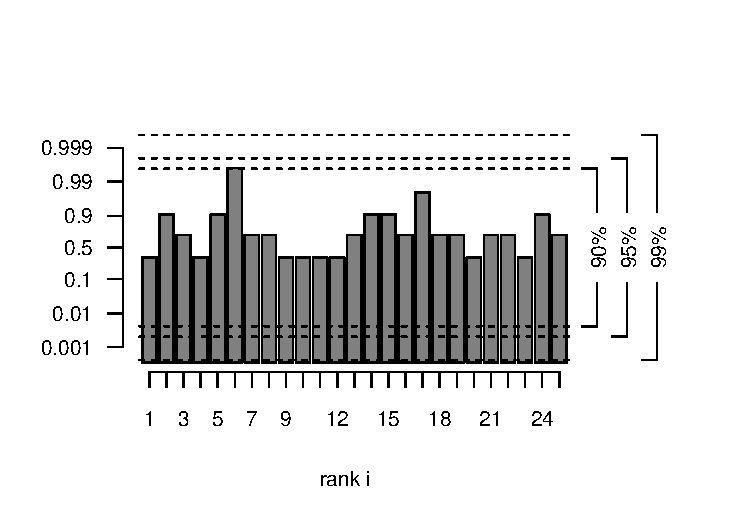
\includegraphics[width=\maxwidth]{figure/rank-hist-pp} 

\end{knitrout}

%
\end{center}
\caption{Rank histogram on probability paper}
\label{fig:rank-hist-pp}
\end{figure}


The function \code{TestRankhist} implements different statistical tests of the null-hypothesis of flat rank histogram.
Flatness of the rank histgram can be assessed by a Pearson $\chi^2$-test \citep{pearson1900criterion}.
Suppose rank $i$ was observed $r_i$ times for $i=1,\dots,R+1$, and define $e_i=N/(R+1)$ the expected number of counts if each verification rank were equally likely.
Define further
\begin{equation}
q_i = \frac{r_i - e_i}{\sqrt{e_i}}.
\end{equation}
%
Under the null-hypothesis of equally likely verification ranks, the test statistic
%
\begin{equation}
\chi^2 = \sum_{i=1}^{R+1} q_i^2
\end{equation}
%
has a $\chi^2$-distribution with $R$ degrees of freedom.


\citet{hamill2001interpretation} showed that certain types of violation of ensemble reliability are visible as different patterns in the rank histogram.
In particular, a systematic bias of the ensemble mean produces sloped rank histograms, and ensembles with insufficient (excessive) ensemble spread produce $\cup$-shaped ($\cap$-shaped) rank histogram.
\citet{jolliffe2008evaluating} showed that the $\chi^2$-test statistic can be decomposed to test for sloped and convex rank histograms specifically, thus increasing the power of the $\chi^2$-test.
The test requires the definition of suitable contrast vectors $\mathbf{c}$ of length $R+1$, that satisfy $\sum_i c_i = 0$, $\sum_i c_i^2 = 1$, and $\sum_i c_i c_i' = 0$ for every pair of contrasts $\mathbf{c}$ and $\mathbf{c}'$.
Assuming a number of up to $R$ contrast vectors $\mathbf{c}^{(1)}$, $\mathbf{c}^{(2)}$, $\dots$, the test statistics $(\sum_i c^{(k)}_i q_i)^2$ are independently $\chi^2$-distributed with one d.o.f. 
The function \code{TestRankhist} applies this test, using a linear and a squared contrast. 
Defining $J=R+1$, the $i$th element of the contrast vectors $\mathbf{c}^{(lin)}$ and $\mathbf{c}^{(sq)}$, for $i=1,\cdots,J$ are given by
%
\begin{align}
c^{(lin)}_i & = -\sqrt{\frac{3(J+1)}{J (J-1)}} + i \sqrt{\frac{12}{J^3 - J}}\text{, and}\\
c^{(sq)}_i & =  - \frac{\sqrt{5}  J^2 - \sqrt{5}}{\sqrt{4(J - 2)  (J-1) J (J+1) (J+2)}}+ \left(i - \frac{J+1}{2}\right)^2   \sqrt{\frac{180}{ J^5 - 5 J^3 + 4 J}}.
\end{align}
%
The $\chi^2$-test using the linear contrast is sensitive to sloped rank histgrams, i.e. biased ensembles, while the $\chi^2$-test using the squared contrast is sensitive to convex rank histograms, i.e. over- or under-dispersed ensemble forecasts.
\code{TestRankhist} returns the test-statistics and one-sided p-values of the Pearson $\chi^2$ test, and of the two tests based on the contrasts $\mathbf{c}^{(lin)}$ and $\mathbf{c}^{(sq)}$:

\begin{knitrout}
\definecolor{shadecolor}{rgb}{0.933, 0.933, 0.933}\color{fgcolor}\begin{kframe}
\begin{alltt}
\hlfunctioncall{TestRankhist}(rh)
\end{alltt}
\begin{verbatim}
##                pearson.chi2 jp.slope jp.convex
## test.statistic      23.9259   0.0114  0.005574
## p.value              0.4658   0.9150  0.940485
\end{verbatim}
\end{kframe}
\end{knitrout}


All p-values are considerably larger than zero.
The rank histogram of the temperature ensemble forecast provides no evidence against the null-hypothesis of a reliable ensemble.

\section{Reliability diagrams for probability forecasts}

The reliability diagram is a classical tool to compare probability forecasts of binary events to the verifying binary observations \citep{wilks2011statistical,jolliffe2012forecast}.
The reliability diagram compares the issued forecast probabilities to the conditional average frequencies of the observation, given the forecast.
A forecast is reliable if the forecast probabilities and their conditional event frequencies are equal.


To estimate the conditional event frequencies the forecast probabilities are grouped into a finite number of non-overlapping bins.
The reliability diagram is a plot of the conditional event frequency per bin over the in-bin average of the forecast probabilities.
\pkg{SpecsVerification} provides the function \code{ReliabilityDiagram} that takes as inputs a collection of probability forecasts and binary verifying observations, and calculates the reliability diagram for a specified number of user-defined bins,  that do not have to be equidistant.
The consistency resampling method proposed by \citet{broecker2007increasing} is used to estimate the expected spread of the reliability diagrams around the diagonal to assess the null-hypothesis that the forecast is reliable.
If the \code{plot} argument is set to \code{FALSE}, the \code{ReliabilityDiagram} function returns the quantities necessary to plot the reliability diagram.
%
\begin{knitrout}
\definecolor{shadecolor}{rgb}{0.933, 0.933, 0.933}\color{fgcolor}\begin{kframe}
\begin{alltt}
p.bin <- \hlfunctioncall{rowMeans}(ens.bin)
\hlfunctioncall{ReliabilityDiagram}(p.bin, obs.bin, plot=FALSE, bins=3)
\end{alltt}
\begin{verbatim}
##   p.avgs cond.probs cbar.lo cbar.hi p.counts bin.lower bin.upper
## 1 0.1713     0.2222  0.0000  0.4784        9    0.0000    0.3333
## 2 0.5833     0.4286  0.1667  1.0000        7    0.3333    0.6667
## 3 0.8447     1.0000  0.6000  1.0000       11    0.6667    1.0000
\end{verbatim}
\end{kframe}
\end{knitrout}

%
If the argument \code{plot=TRUE} the reliability diagram is plotted, as shown in Figure \ref{reldiag-plot}. 
The logical argument \code{plot.refin} controls the refinement diagram, i.e. the histogram over the forecast probabilities.
The logical argument \code{attributes} controls plotting of the polygon defined by the vertical no-resolution line at $\bar{y} = 1/n \sum_t y_t$, where $y_t$ is the binary observation at time $t$, and the no-skill line defined by the linear equation $f(x)=(x+\bar{y})/2$, to produce the attributes diagram \citep{hsu1986attributes}.
Points that fall into the shaded area of the attributes diagram contribute positively to forecast skill (defined by the Brier skill score).

\begin{figure}
\begin{center}
%
\begin{knitrout}
\definecolor{shadecolor}{rgb}{0.933, 0.933, 0.933}\color{fgcolor}\begin{kframe}
\begin{alltt}
rd <- \hlfunctioncall{ReliabilityDiagram}(p.bin, obs.bin, plot=TRUE, bins=3, attributes=TRUE)
\end{alltt}
\end{kframe}
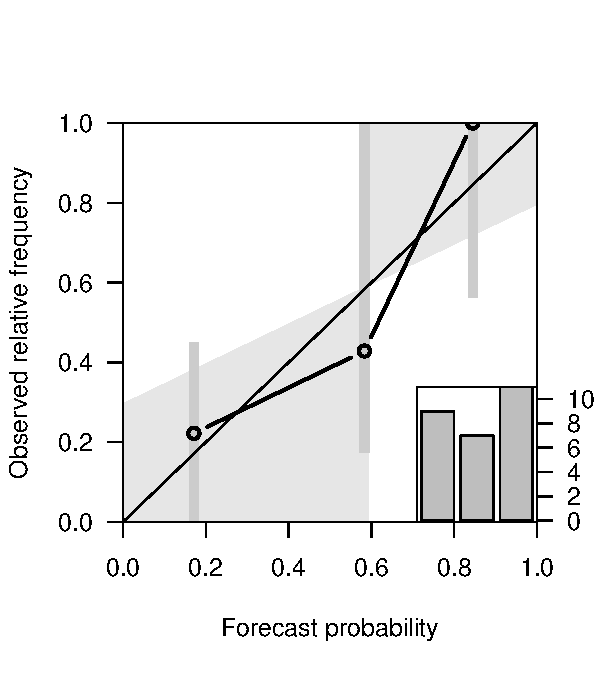
\includegraphics[width=\maxwidth]{figure/reldiag} 

\end{knitrout}

%
\end{center}
\caption{Reliability diagram of temperature exceedance forecasts \code{p.bin}, using 3 equidistant bins to estimate the conditional event frequencies.} 
\label{reldiag-plot}
\end{figure}


\section{Additional functions}

The focus of \pkg{SpecsVerification}, and of the present paper, is on verification functions for ensemble and probability forecasts, uncertainty quantification, and graphical display of the results.
\pkg{SpecsVerification} includes a number of functions for post-processing and forecast verification that were included following user requests.


For verification of deterministic forecasts $x_t$ , e.g. the ensemble mean forecast, the squared error score $(x_t - y_t)^2$ (function \code{SqErr}), and the Absolute Error score $|x_t - y_t|$ (function \code{AbsErr}) have been implemented.
The function \code{GaussCrps} calculates the CRPS (eq.~\ref{eq:crps}) where the forecast cdf $F_t(x)$ is a Normal distribution with mean $\mu_t$ and standard deviation $\sigma^2_t$.
The CRPS integral can then be solved analytically \citep{gneiting2005calibrated} thus eliminating the need for expensive numerical integration.
These score functions be analysed by the functions \code{ScoreDiff} and \code{SkillScore}.


Ensemble forecasts produced by numerical climate models often contain systematic errors due to numerical approximations, missing physical mechanisms in the model, or coding errors.
These biases include a constant bias of the mean, or ensemble dispersion errors.
Ensemble dressing is a statistical post-processing method based on kernel density estimation to transform a raw forecast ensemble into a smoothed probability distribution function.
In particular, affine kernel dressing \citep[AKD; ][]{broecker2008from} is a method that corrects systematic model errors by an affine transformation of the ensemble, and produces a smooth forecast distribution by dressing the transformed ensemble members with Gaussian kernels.
AKD is implemented in the function \code{DressEnsemble}, and the AKD parameters can be fitted with the function \code{FitAkdParameters}. 
The dressed ensemble can be evaluated by the CRPS using the function \code{DressCrps} which uses results by \citet{grimit2006the}, and by the Ignorance Score \citep{roulston2002evaluating}, also known as the Logarithmic score, using the function \code{DressIgn}.
The dressed ensemble can be further analysed by the functions \code{GetDensity} and \code{PlotDressedEns}.

Auxiliary functions were added to the package, namely the function \code{Detrend} to remove a common linear trend from an ensemble of forecasts, and the function \code{GenerateToyData} that simulates artificial ensemble and observation data using a statistical signal-plus-noise model \citep{siegert2016bayesian}.




\section{Conclusion}

The package \pkg{SpecsVerification} for the \proglang{R} statistical programming environment implements a variety of forecast verification functions that are not available in previous verification software packages.
The focus of \pkg{SpecsVerification} is on comparative verification of ensemble forecasts, and uncertainty quantification by statistical testing and confidence intervals.
Continuous, categorical and binary ensemble forecasts for univariate quantities can be evaluated and compared by a number of verification scores.
Additional functions for data transformation and statistical post-processing simplify a number of common verification tasks.


\section*{Acknowledgements}

This paper has benefitted from numerous discussions with the members of the statistical science group at the University of Exeter, in particular Chris Ferro and David Stephenson.
This work was supported by the European Union Programme FP7/2007-13 under grant agreement 3038378 (SPECS).
The views expressed herein are those of the author and do not necessarily reflect the views of funding bodies and their subagencies.


\bibliography{ensemble-verification}

\end{document}
